\documentclass[12pt,a4paper]{article}

\usepackage[utf8]{inputenc}
\usepackage[T1]{fontenc}
\usepackage[ngerman]{babel}

\usepackage[autostyle=true,german=quotes]{csquotes}

\usepackage{hyperref}
\usepackage{url}

\hypersetup{
	pdftitle    = {Die Geschichte der Deutschen Demokratischen Republik},
	pdfsubject  = {Die Geschichte der Deutschen Demokratischen Republik},
	pdfauthor   = {Yannik Bürkle}
}

\usepackage{graphicx}

\usepackage[style=authortitle,backend=biber]{biblatex}
\addbibresource{quellen.bib}

\title{Die Geschichte der Deutschen Demokratischen Republik}
\author{Yannik Bürkle}
\date{19. Dezember 2016}

\begin{document}
\maketitle
\newpage



\begin{quotation}
    \enquote{Während die Menschen in der Sowjetischen Besatzungszone mit den Härten ihres Alltags rangen, organisierte eine kleine Gruppe von Kommunisten die Machtübernahme. So entstand die DDR.} \\
    \textit{aus SPIEGEL Geschichte 3/2015: Die DDR - Leben im sozialistischen Deutschland}
\end{quotation}



\newpage



\tableofcontents



\newpage



\section{Einleitung}
\label{sec:einleitung}



Die Deutsche Demokratische Republik war ein Staat, der am 7. Oktober 1949 durch die Teilung Deutschlands aus der Sowjetischen Besatzungszone hervorging und bis zum 3. Oktober 1990 existierte. Die DDR war ein kommunistischer Staat unter der Führung der Sozialistischen Einheitspartei.\footcite{wiki:ddr}



\newpage



\section{Die Aufteilung Deutschlands (1945 - 1949)}
\label{sec:die-aufteilung-deutschlands}
Der Initiator für eine Aufteilung Deutschlands war der Zweite Weltkrieg. Nach der Kapitulation der Wehrmacht am 7. bzw. 8. Mai 1945 wurde die \enquote{Deutschlandfrage} besprochen.\footcite{wiki:teilung} Auf den Außenministerkonferenzen der vier Siegermächte in Moskau und London konnte keine Einigung getroffen werden. Die USA, Frankreich und Großbritannien entschieden sich für eine Weststaatslösung.\footcite{umbruch} 

Außerdem wurde auf den Konferenzen von Teheran und Jalta eine Teilung Deutschlands diskutiert. Im Juli 1945 wurden diese Pläne auf der Potsdamer Konferenz erstmals konkretisiert. Deutschland sollte in vier Besatzungszonen (Abb.~\ref{img:besatzungszonen}) aufgeteilt, aber von einem gemeinsamen Aliiertenkontrollrat verwaltet werden.\footcite{wiki:teilung}

\begin{figure}[h]
	\centering
	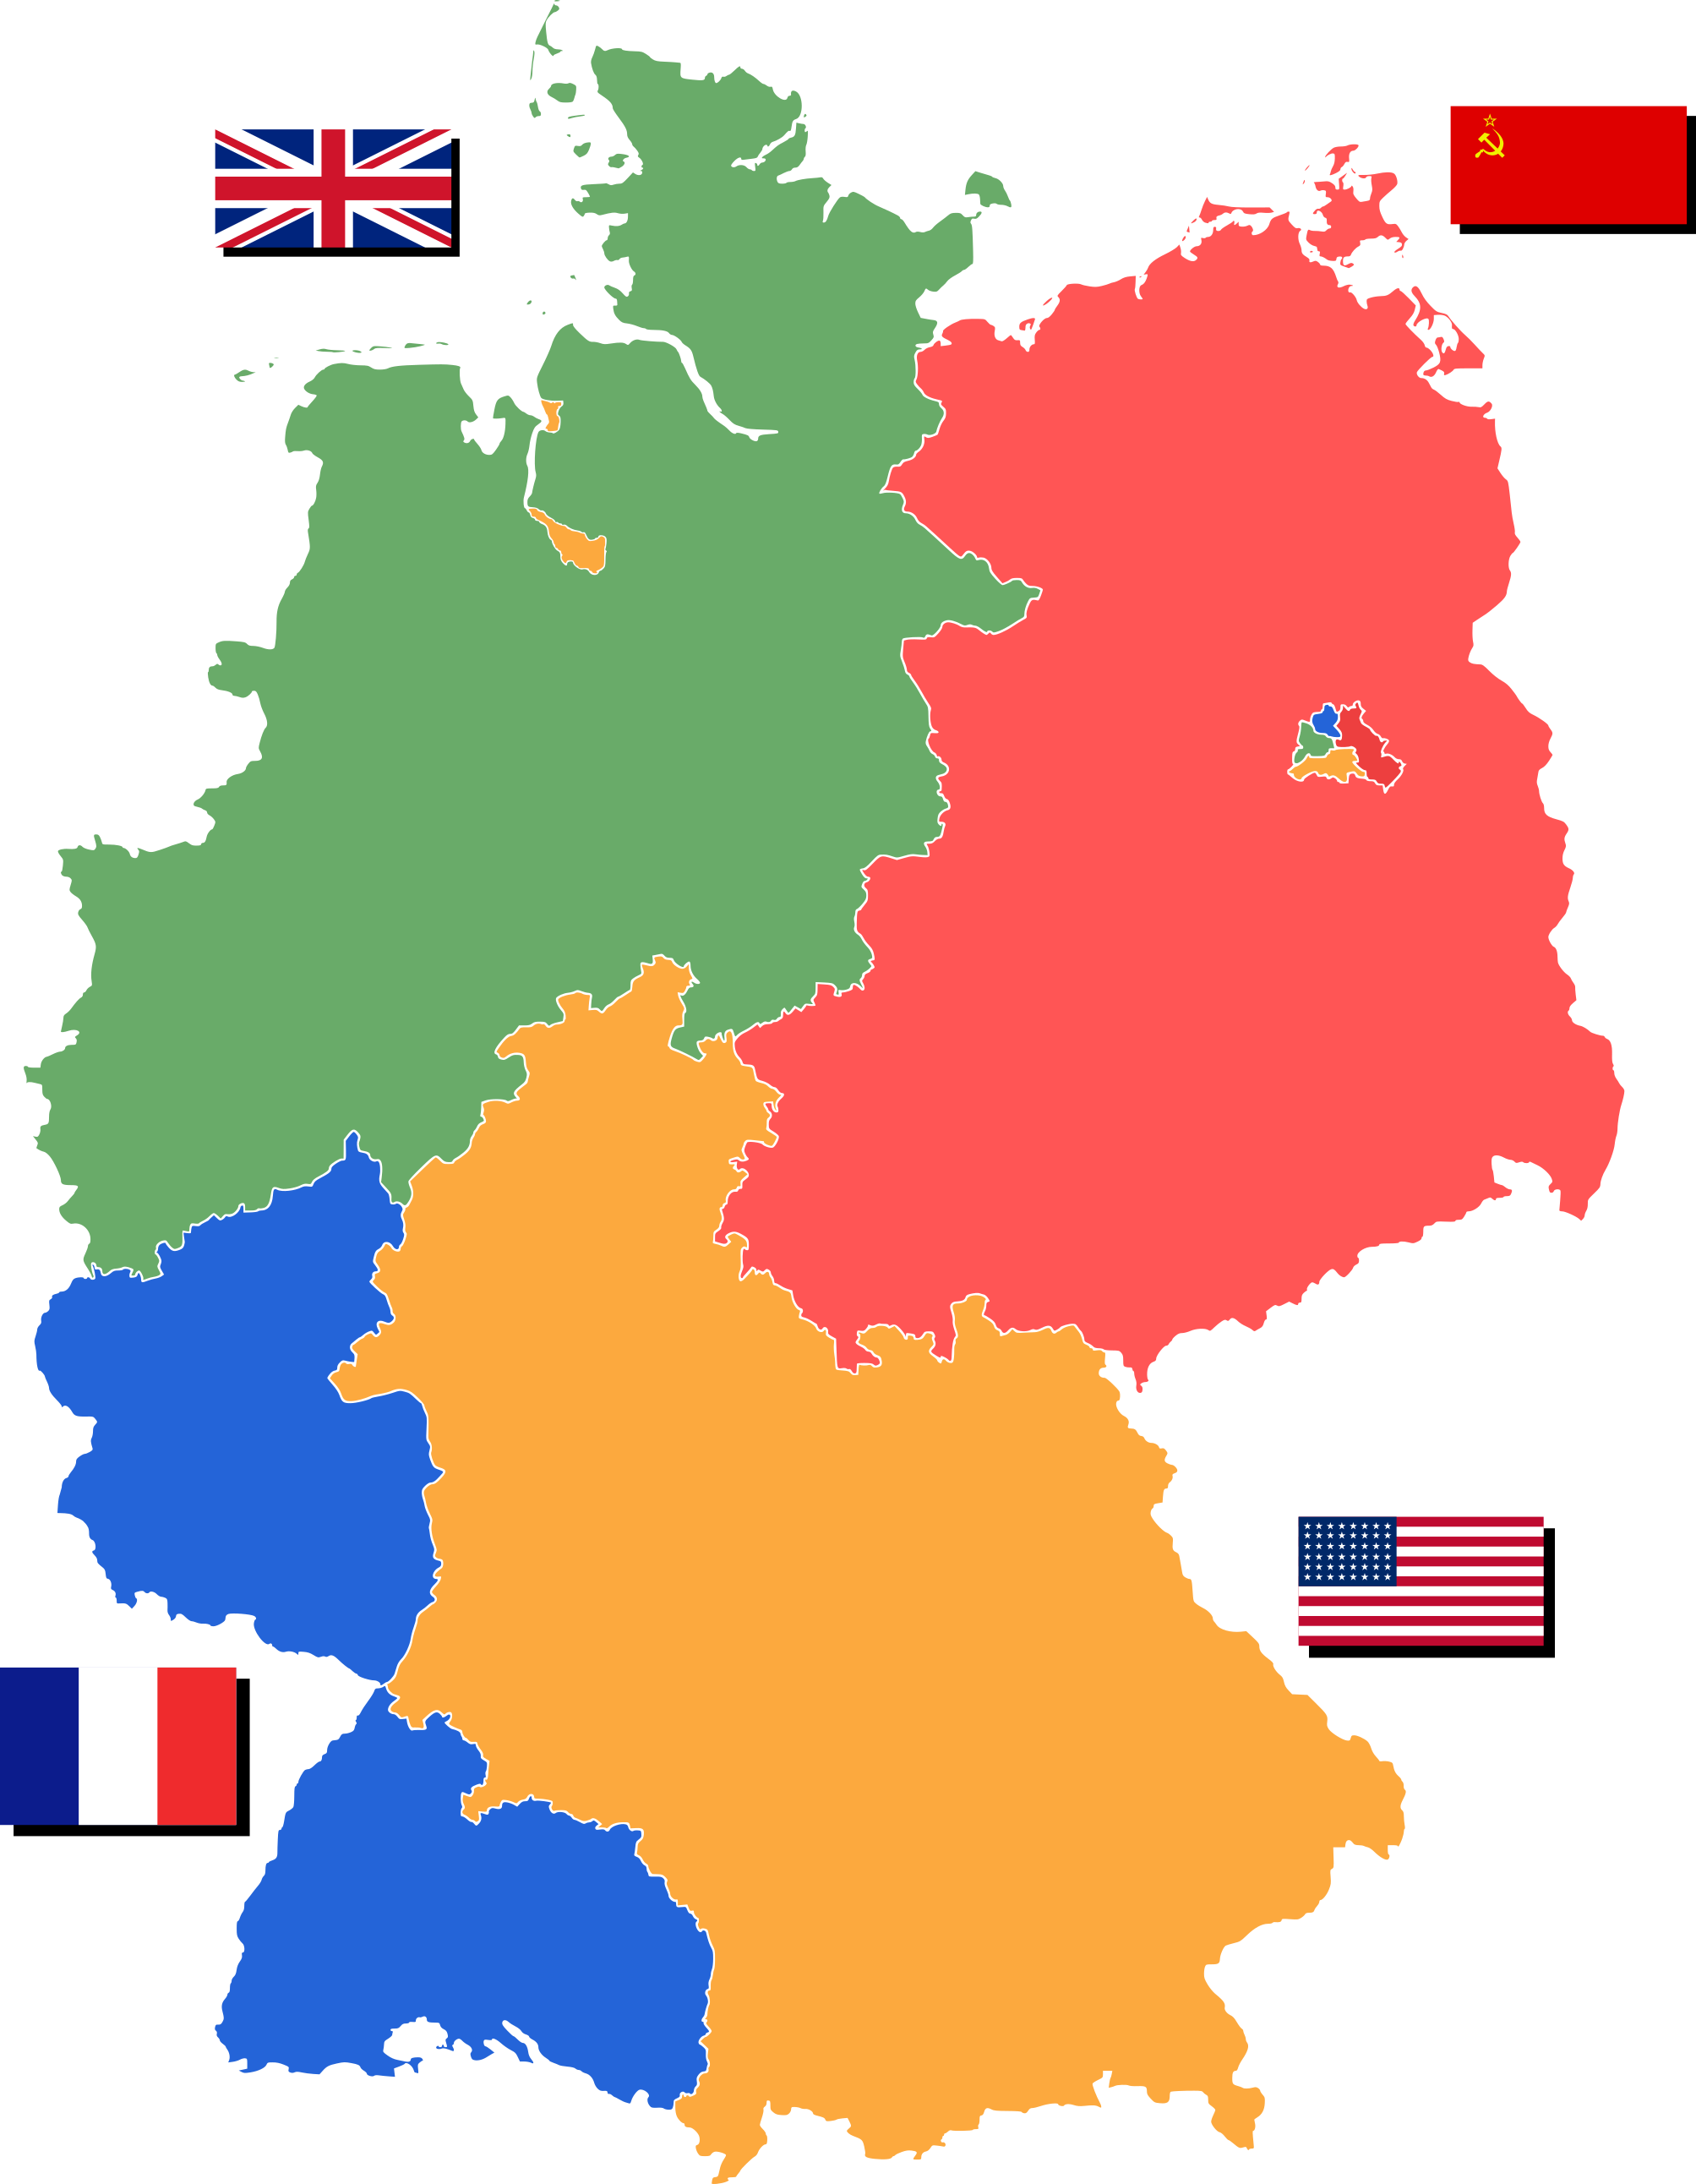
\includegraphics[width=0.5\textwidth]{Bilder/Besatzungszonen.png}
	\caption{Die vier Besatzungszonen und Berlin}
	Quelle: Wikipedia
	\label{img:besatzungszonen}
\end{figure}

Die wirtschaftlichen Entwicklungen zwischen den westlichen Besatzungszonen und der Sowjetische Besatzungszone gingen jedoch schnell stark auseinander. Außerdem kam es im Kalten Krieg zu steigenden Spannungen zwischen Ost und West.
1947 schlossen sich daher die Britische und Amerikanische Zone zur sogenannten \enquote{Bizone} zusammen. Die USA beschloss den Marshallplan zur materiellen Stärkung des Westens Deutschlands und Schwächung des kommunistischen Einflusses in Westeuropa.\footcite{izpb:weg-diktatur} 

Währenddessen setzte die SBZ die Demontagen fort und verhinderte die Einbindung in den Marshallplan\footnote{Eigentlich: \enquote{Europäisches Wiederaufbauprogramm} nach C. Marshall}. Dies hätte nämlich unter anderem die Einbindung in das westliche Wirtschaftssystem bedeutet.

Auf einer Aliiertenkonferenz trugen die Westaliierten ihren Plan zur Gründung eines Westdeutschen Separatstaates vor. Ein Vertreter der SBZ verließ daraufhin den Versammlungsraum, da er eine Teilung Deutschlands befürchtete.

In Westberlin wurde die westliche Währung eingeführt. Da dies gegen des Willens der SBZ geschah, wurde eine \enquote{Berlin-Blockade} errichtet. Bis zum Mai 1949 wurde Berlin ganze 11 Monate über eine Luftbrücke mit Lebensmitteln versorgt.


\subsection{Einwirkungen der Sowjetunion}
\label{aufteilung:einwirkungen-udssr}

Während des Zweiten Weltkrieges entwickelte Josef Stalin eigene Ideen für ein Nachkriegsdeutschland. Ihm schwebte ein ungeteilter, neutraler und nichtsozialistischer Staat vor. Er erwartete, dass die Sowjetunion Reparationszahlungen aus dem Ruhrgebiet erhielt. Im Gegenzug sollten Nahrungsmittel aus der SBZ indie westlichen Zonen fließen. Da es seitens der SBZ jedoch nie zu Lieferungen kam, wurden die Zahlungen des Ruhrgebiets eingestellt.

Diese Pläne konnte Stalin also nicht durchsetzen. Er verschob die \textit{Sowjetisierung} und vertuschte eine kommunistische Entwicklung, da er in jedem Falle den Eindruck vermeiden wollte, die Sowjetunion sei schuld an der Teilung Deutschlands. Die SED sollte nach außen weiterhin Interesse an einer gesamtdeutschen Lösung zeigen. Innenpolitisch sollte sie jedoch alles für die Abspaltung vorbereiten.\footcite{izpb:weg-diktatur}

Die Sowjetunion setzte in der SBZ die \textit{Sowjetische Militäradministration in Deutschland (SMAD)} ein. Diese sollte den Aufbau eines politischen Systems im Sinne der Sowjetunion steuern und die Besatzungszone verwalten. Weiterhin kontrollierte und regelte sie das gesamte politische und gesellschaftliche Leben.\footcite{wiki:ddr}



\newpage



\section{Die Anfänge (1949 - 1961)}
\label{sec:die-anfaenge}


\subsection{Vorbereitungen}
\label{anfange:vorbereitungen}

Da deutschlandpolitische Übereinkünfte zwischen den Aliierten endgültig scheiterten, bestand für die Führungsebene der SED keine Notwendigkeit mehr zu außerpolitischen Rücksichtnahmen. Sie entschied sich daher die Bildung eines Ostdeutschen Teilstaates abzuschließen. Ein Problem war jedoch, dass die SED nie wirklich politisch legitimiert war.\footnote{Sie wurde nie vom Volk in offener Wahl gewählt.} Die SED schug vor, einen \enquote{Deutschen Volskongreß} wählen zu lassen.\footcite{izpb:ausbau-system}

Am 15. und 16. Mai 1949 wurde der 3. Volkskongress über Einheitslisten gewählt. Die Wahlbeteiligung lag bei 94,1 Prozent.\footcite{izpb:ausbau-system} Als sich nach etwa der Hälfte der Stimmenauszählung keine Mehrheit für \enquote{Ja} abzeichnete, wurde entschieden alle durchgestrichenen oder leeren - also alle ungültigen - Stimmzettel als \enquote{Ja} zu werten. Das offizielle Ergebnis vom 16. Mai 1949 besagte daher 66,1\% der Abstimmenden befürworteten die Einheitslisten.

Am 29. Mai wählte der Kongress einen Deutschen Volksrat, der bereits einen Tag später einen Entwurf einer Verfassung für die Deutsche Demokratische Republik präsentierte. Der rechtliche Rahmen des künftigen Staats war damit bereits abgesteckt.


\subsection{Staatsgründung}
\label{anfaenge:staatsgruendung}

\begin{figure}
    \centering
    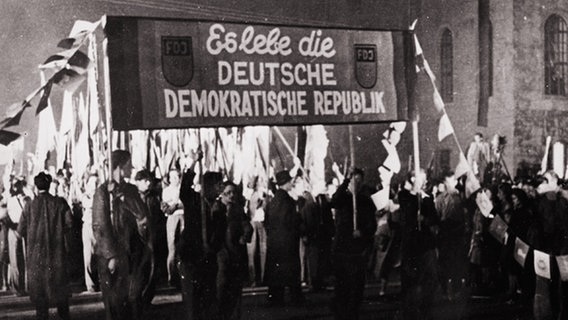
\includegraphics[width=0.7\textwidth]{Bilder/gruendungddr102_v-contentgross.jpg}
    \caption{\enquote{Es lebe die Deutsche Demokratische Republik} - Staatlich inszenierte Kundgebungen in Berlin}
    Quelle: \url{ddr-geschichte.de}
    \label{img:gruendung}
\end{figure}

Mitte September 1949 besprach eine SED-Delegation die konkreten Schritte zur Gründung des Teilstaates in Moskau. Am 7. Oktober formten sich die 330 Mitglieder des Volksrats zur \enquote{provisorischen Volkskammer der Deutschen Demokratischen Republik} zusammen. Die SED hatte mit 96 Abgeordneten den größten Teil. Noch an diesem Tag beschloss die Volkskammer das Inkrafttreten der neuen Verfassung als \enquote{Akt der Staatsgründung}~(\cite{izpb:ausbau-system}). 

Am 11. Oktober wurde \textit{Wilhelm Pieck (s. Abb. \ref{img:pieck})} zum Staatspräsidenten gewählt. Zum Regierungschef ernannt wurde \textit{Otto Grotewohl (s. Abb. \ref{img:grotewohl})}. Beide waren damals Vorsitzende der SED. Walter Ulbricht wurde Vorsitzender des Zentralkomitees

Die Verfassung beschrieb allerdings keine Gewaltenteilung, sondern eine \textbf{Gewaltenkonzentration} in diversen SED-Organen.

\begin{figure}
    \centering
    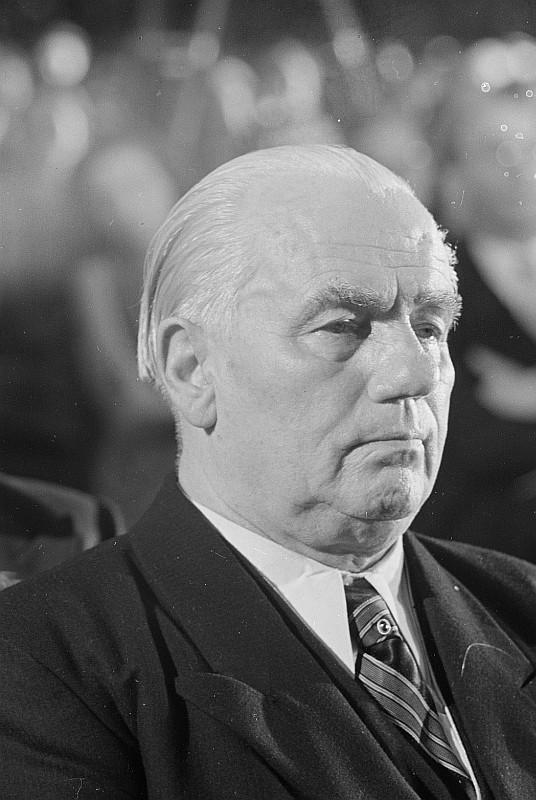
\includegraphics[width=0.3\textwidth]{Bilder/Wilhelm-Pieck.jpg}
    \caption{Wilhelm Pieck, erster Staatspräsident der DDR}
    Quelle: Wikipedia
    \label{img:pieck}
\end{figure}

\begin{figure}
    \centering
    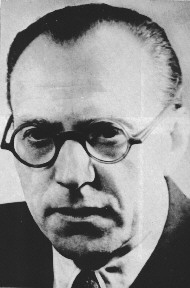
\includegraphics[width=0.3\textwidth]{Bilder/Otto-Grotewohl.jpg}
    \caption{Otto Grotewohl}
    Quelle: \url{ddr-geschichte.de}
    \label{img:grotewohl}
\end{figure}


\subsection{Wirtschaft}
\label{anfaenge:wirtschaft}

Die Wirtschaft der Deutschen Demokratischen Republik war bereits von Anfang an stark durch die Demontage seitens der Sowjetunion beeinflusst. Josef Stalin ließ bis 1946 über 1.000 Betriebe abbauen, vor allem der Branchen Maschinenbau, chemischer und optischer Industrie. Außerdem wurden an nahezu allen Bahnstrecken die Elektrifizierungen und das zweite Gleis abgebaut.

460 Betriebe wurden in Staatseigentum der Sowjetunion als \textit{Sowjetische Aktiengesellschaften} überführt.

Abgebaut wurden
\begin{itemize}
    \item 82\% der Walzwerke,
    \item 80\% der Eisenproduktion,
    \item 75\% der Hohlziegelerzeugung,
    \item 45\% der Papiererzeugung,
    \item 45\% der Zementherstellung,
    \item 35\% der Energieerzeugung,
    \item 30\% der Schuhindustrie,
    \item 25\% der Textilindustrie und
    \item 25\% der Zuckerproduktion
\end{itemize}

Insgesamt waren durch die Demontage etwa 75 Prozent der ostdeutschen Kapazitäten betroffen und die DDR war in der Industrialisierung wieder auf dem Stand vor 1936.
Offiziell wurden an die UdSSR etwa 4,3 Millionen US Dollar gezahlt, Schätzungen zufolge waren es eher 15 bis 18 Millionen US Dollar.\footcite{wiki:geschddr}


\subsubsection{Fünfjahrplan}
\label{fuenfjahr}

Im Jahr 1950 wurde die Zentrale Plankommission gegründet, die die zentrale wirtschaftliche Lenkung der DDR übernahm.
Sie schuf einen Fünfjahrplan von 1951 bis 1955, der die Wirtschaft \enquote{vorwärts zu neuen Erfolgen} \textit{(Abb. \ref{img:fuenfjahrplan})} führen sollte. Sie enthielten Zuweisungen von Fonds und Ressourcen und Vorgaben für zu erbringende Produktion und Dienstleistungen.\footcite{wiki:fuenfjahrplan}.

\begin{figure}[hbp]
    \centering
    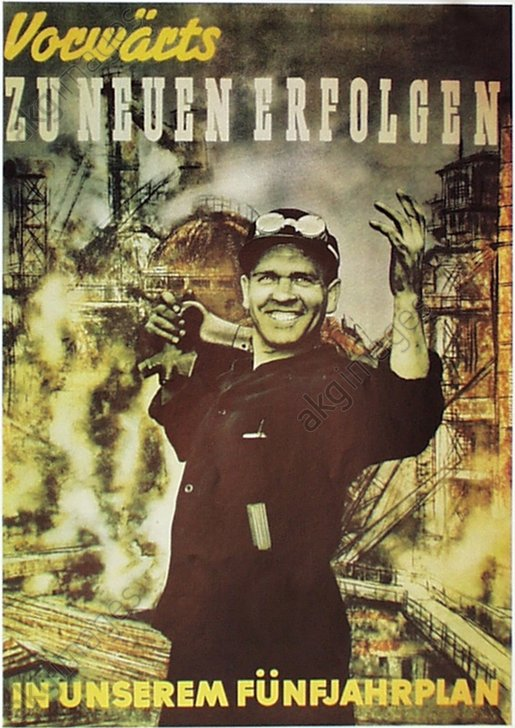
\includegraphics[width=0.5\textwidth]{Bilder/fuenfjahrplan.jpg}
    \caption{\enquote{Vorwärts zu neuen Erfolgen}}
    Quelle: akg images
    \label{img:fuenfjahrplan}
\end{figure}


1958 wurden die damals üblichen Lebensmittelkarten (Abb. \ref{img:lebensmittel}) endgültig abgeschafft. Zahlreiche Betriebe wurden aus den Sowjetischen Aktiengesellschaften (vgl. \ref{anfaenge:wirtschaft}) von der DDR zurückgekauft und in \textit{Volkseigene Betriebe} umgewandelt.

\begin{figure}[hbp]
    \centering
    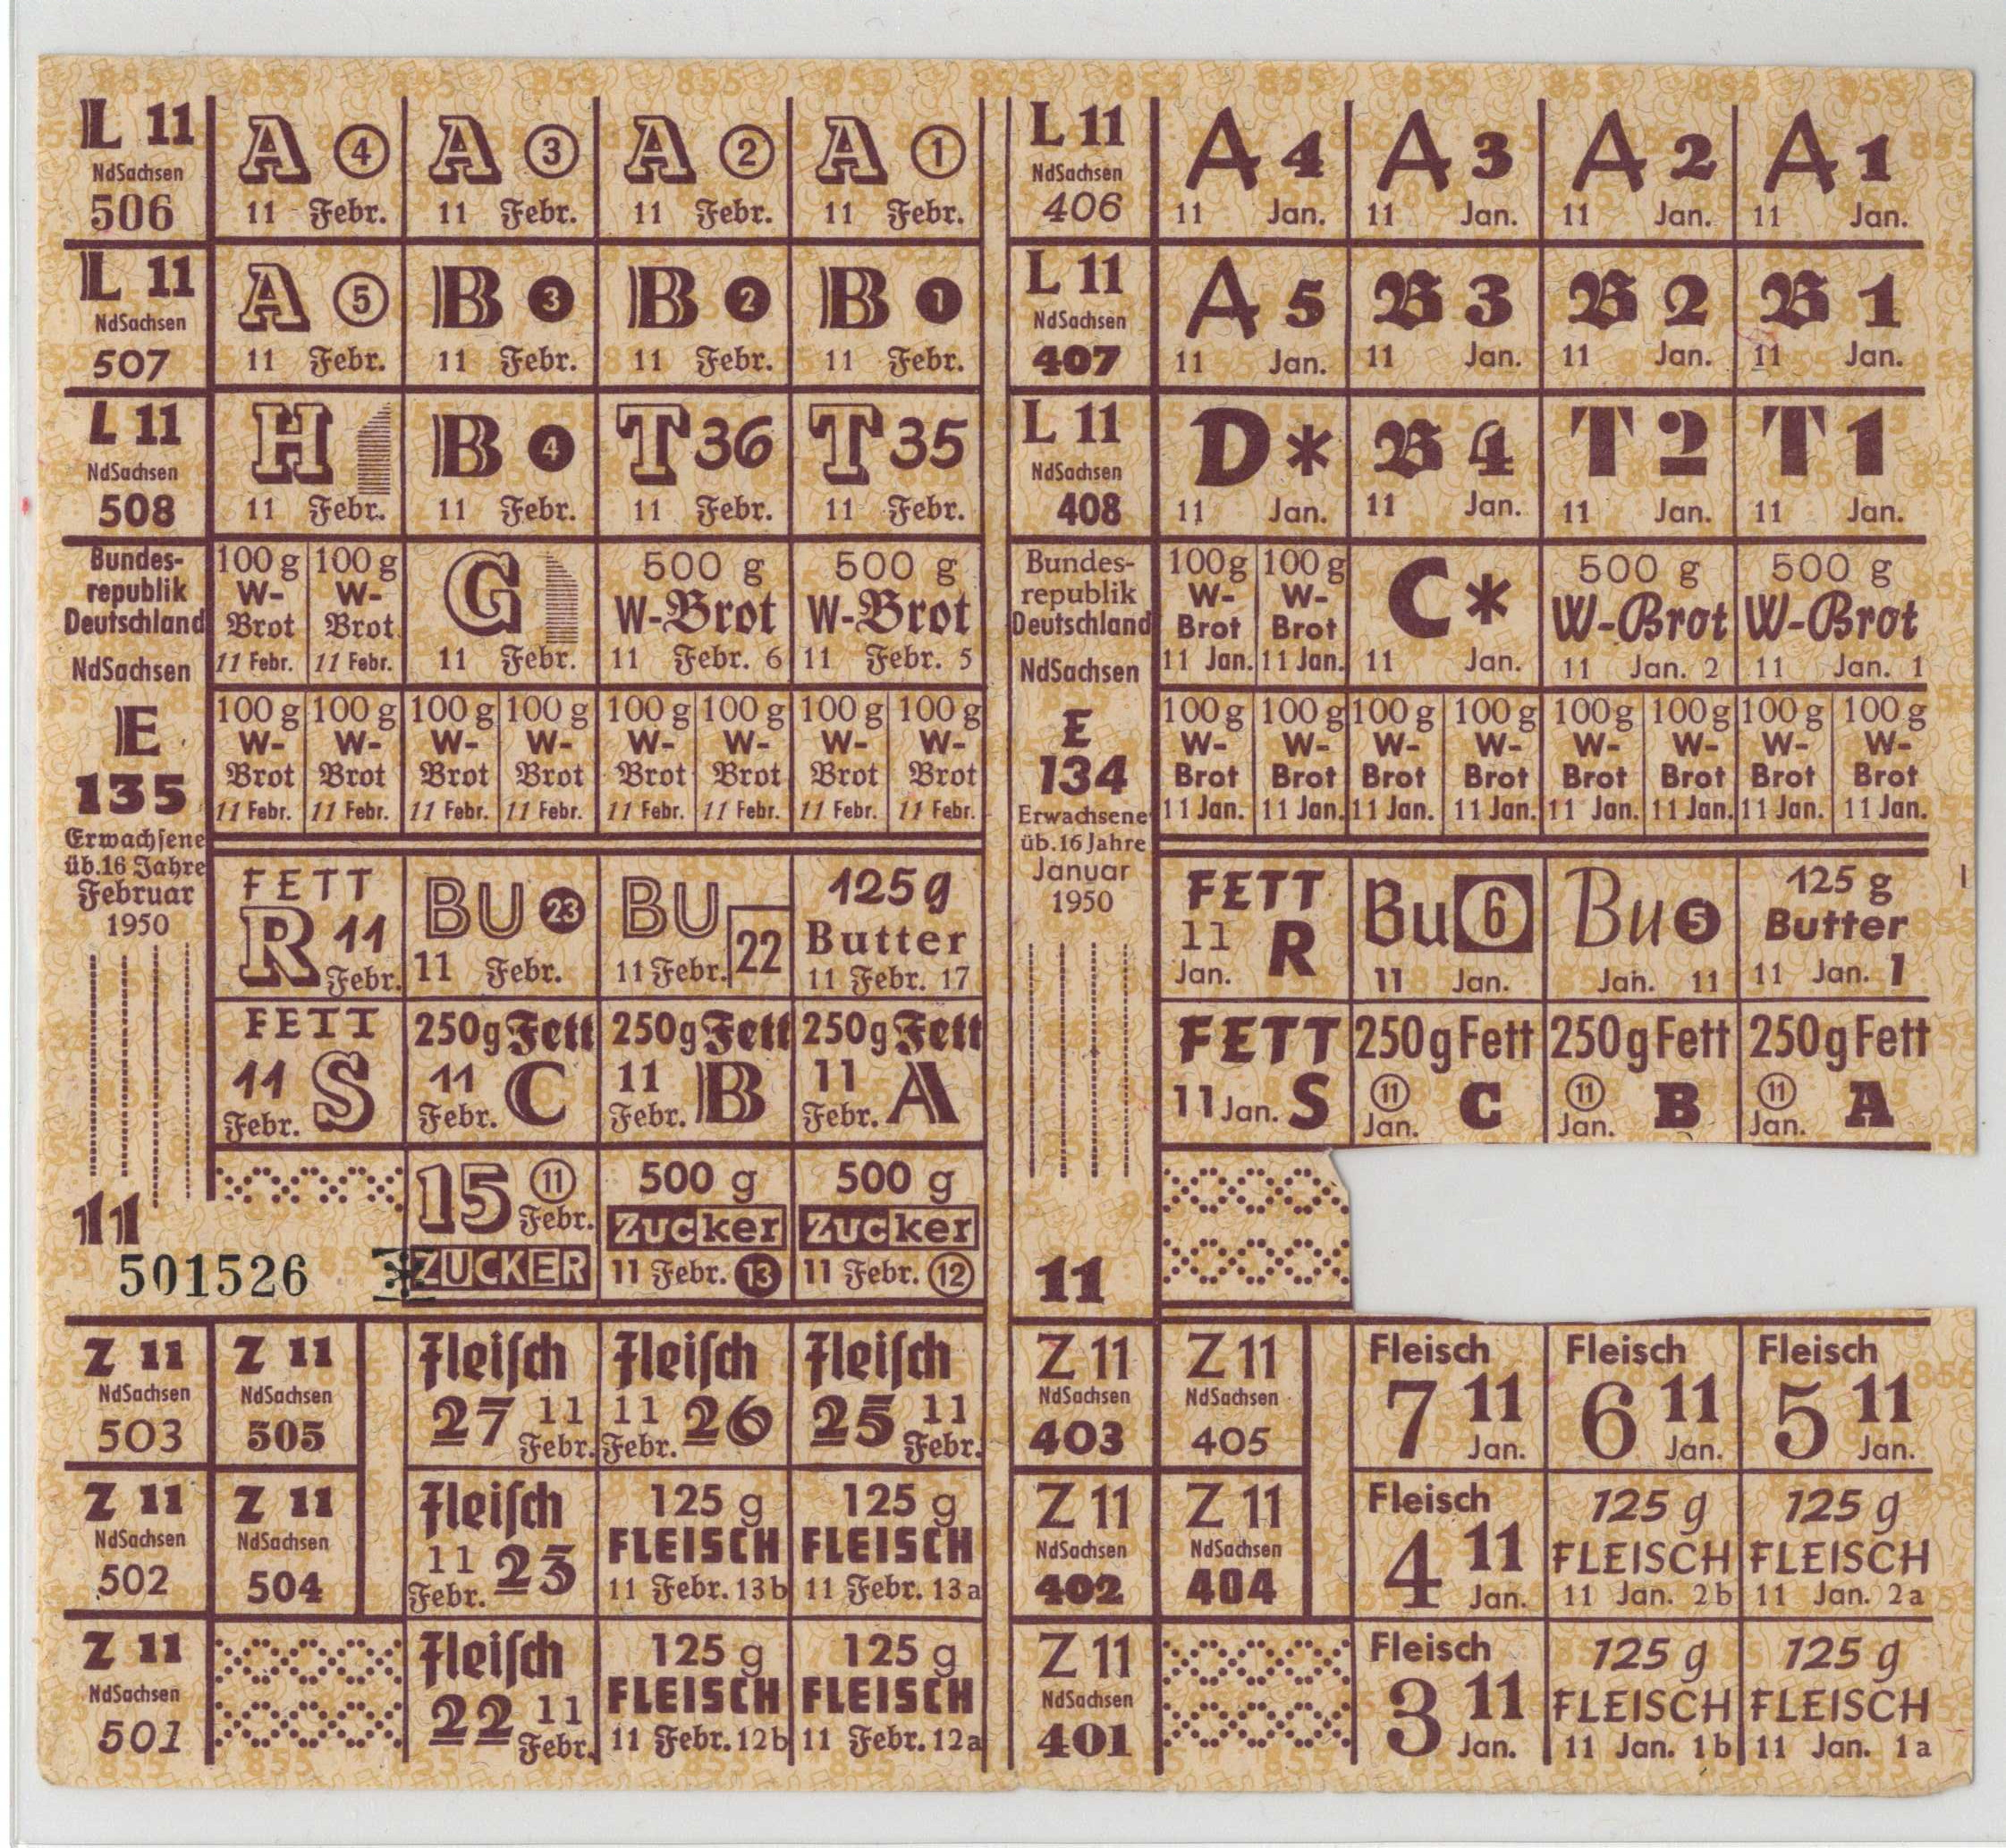
\includegraphics[width=0.6\textwidth]{Bilder/Lebensm1.JPG}
    \caption{Lebensmittelkarte}
    Quelle: Wikipedia
    \label{img:lebensmittelk}
\end{figure}


\subsubsection{Landwirtschaft}
\label{landwirtschaft}

Die Landwirtschaft der DDR wurde stark von der Devise \enquote{Vom Ich zum Wir} geprägt. Die SED-Führung versuchte die Landwirte \enquote{auf freiwilliger Basis} von einer kollektiven Landwirstschaft zu überzeugen. Es wurden \enquote{Landwirtschaftliche Produktionsgenossenschaften} gegründet, welche die Idee der Sowjetisierung überall hin tragen sollten. 1952 gab es bereits knapp 2.000 solcher LPGs. Die meisten darunter bestanden aus wirtschaftsschwachen Landwirten, da kleine Bauern mit hohen Zwangsabgaben drangsaliert und einer schlechteren Vergabe der MAS benachteiligt wurden. Aus folge dessen flohen in den Anfangsjahren etwa 10.000 Bauern in den Westen.


\subsection{Weitere Entwicklungen}
\label{anfaenge:weiter}

Walter Ulbricht wurde zum Generalsekretär des neu geschaffenen Zentralkomitees der SED. Nach dem Tod von Wilhelm Pieck wurde das Amt des Präsidenten abgeschafft und das Zenralkomitee (ZK) - mit Walter Ulbricht als Vorsitzenden - zum höchsten Amt der DDR heraufgestuft.

In den Wahlen zur Volkskammer erreichte die SED in den folgenden Jahren 99,3\%, 99,5\% bzw. 99,7\% der Stimmen.


\subsection{Ost und West}
\label{anfaenge:ost-west}

Am 10. März 1952 bot Josef Stalin in den \textit{Stalin-Noten} Verhandlungen über die Wiedervereinigung Deutschlands an. Die Westmächte gingen von einem Ablenkungsmanöver aus, weshalb sie die Verhandlung ignorierten. Es kam also zu keinem Ergebnis in Sachen Wiedervereinigung, sondern zum genauen Gegenteil: Die Ostintegration und Sozialisierung der DDR wurde vorangetrieben.\footcite{stalinnoten}\footcite{wiki:geschddr}

Im Jahr 1954 wurde die Bundesrepublik Mitglied der Westeuropäischen Union und der NATO\footnote{North Atlantic Treaty Organization}. Als Antwort darauf trat am 14. Mai 1955 die DDR dem Warschauer Pakt \textit{(\enquote{Vertrag über Freundschaft, Zusammenarbeit, und gegenseitigen Beistand})} bei. Für die DDR ist dies ein weiterer Schritt zur Anerkennung unter den \enquote{sozialistischen Bruderstaaten}.\footcite{warschauer-pakt}


\subsection{Flucht aus der DDR}
\label{flucht}

\begin{table}[hh]
    \begin{center}
        \begin{tabular}{ c c c }
            \hline
            \hline
            \bf Jahr & \bf Personen & \bf davon Jugendliche unter \\
            & & \bf 25 Jahre in Prozent \\
            \hline
            1949 & 129.245 & - \\
            1950 & 197.788 & - \\
            1951 & 165.648 & - \\
            1952 & 182.393 & - \\
            1953 & 331.390 & 48,7 \\
            1954 & 184.198 & 19,1 \\
            1955 & 252.870 & 49,1 \\
            1956 & 279.189 & 49,0 \\
            1957 & 261.622 & 52,2 \\
            1958 & 204.092 & 48,2 \\
            1959 & 143.917 & 48,3 \\
            1960 & 199.188 & 48.8 \\
            1961 & 207.026 & 49.2 \\
            \hline
            \hline
        \end{tabular}
    \end{center}
    \caption{Flüchtlinge aus der DDR und dem Ostsektor von Berlin 1949-1961}
    Quelle: Informationen zur politischen Bildung Nr. 312/2011\footcite{izpb:ausbau-system}
\end{table}

Die DDR musste bereits seit Beginn mit einer großen Abwanderung kämpfen. Bis 1956 sind 1,72 Millionen Menschen geflohen. Unter den Flüchtlingen waren auch viele gut ausgebildete Menschen. Durch deren Fehlen schwächte sich die Wirtschaftskraft der DDR und bedrohte deren Existenz.

Durch ein neues Passgesetz wurde die \enquote{Republikflucht} kriminalisiert.

Im Jahr 1952 wurden \enquote{unzuverlässige Bürger}, die nahe der innerdeutschen Grenze wohnten, durch die Aktion \enquote{\textbf{Ungeziefer}} ins Hinterland umgesiedelt.
1954 baute die DDR eine fünf Kilometer breite Sperrzone bestehend aus einem 500 Meter breiten Schutzstreifen mit stacheldraht und einem zehn Meter breiten Kontrollstreifen.

Die Zeichen einer Staatskrise häufte sich im Jahre 1960 erneut. Die eigenen Ziele der Regierung konnten nicht erreicht werden, darunter die Bestrebungen, die Bundesrepublik im Lebensstandard zu übertreffen.
1960 kam es zu erheblichen Wirtschaftseinbrüchen, obwohl es die Jahre zuvor bergauf ging.\footcite{izpb:ausbau-system}

\subsubsection{Bau der Mauer}
\label{bau-der-mauer}

\begin{figure}[h]
    \centering
    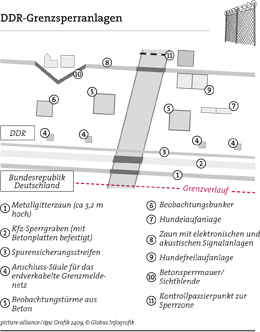
\includegraphics[width=0.3\textwidth]{Bilder/Grenze-Schema.jpg}
    \caption{DDR-Grenzsperranlagen: Schematische Zeichnung}
    Quelle: Bundeszentrale zur politischen Bildung
    \label{img:grenze-schema}
\end{figure}

Am 13. August 1961 wurde mit dem Beginn der Berliner Mauer begonnen. Dies war der verzweifelte Versuch der SED-Führung, den drohenden Kollaps zu verhindern. Walter Ulbricht forderte, die Fluchtbewegung gewaltsam zu stoppen.
Nach außen versuchte er, dies zu dementieren, indem er am 15. Juni 1961 auf einer Pressebewegung sagte:

\begin{quotation}
    \enquote{Niemand hat die Absicht eine Mauer zu bauen.}
\end{quotation}

Kurz darauf wurde der Forderung Ulbrichts entsprochen und Schießbefehl gegen Flüchtige erlassen. Ab 1962 verminte die DDR ihre Seite der Grenze.



\newpage



\section{Stabilisierungsphase (1961 - 1980)}
\label{sec:stabilisierungsphase}

Am 20. Februar 1967 verabschiedete die Volkskammer das Gesetz über die Staatbürgerschaft. Die Staatsbürgerschaft der DDR löste die bisherige Deutsche Staatsbürgerschaft ab.

Nach einer Volksabstimmung, die nach eigenen Angaben eine Zustimmung von 96,37 Prozent der abgegebenen Stimmen [...] erbracht hatte, trat im April 1968 eine neue Verfassung in Kraft.\footcite[wörtl. aus][]{izpb:reform}
In dieser Verfassungsänderung wurde die DDR zum \enquote{sozialistischen Staat deutscher Nation}, die BRD zum kapitalistischen Teil. Außerdem wurde die Führungsrolle der Sozialistischen Einheitspartei festgeschrieben.


\subsection{Ende der Ära Ulbricht}
\label{ende-ulbricht}

Nach einem Streit zwischen Walter Ulbricht und der Parteiführung, seine Reformen und Ansichten betreffend. Daraufhin wurde Ulbricht gezwungen, \enquote{aus gesundheitlichen Gründen} von all seinen Ämtern zurückzutreten. Am 3. Mai 1971 endete damit die Ära Ulbricht.

Sein Nachfolger als Erster Sekretär des Zentralkomitees wurde Erich Honecker (Abb. \ref{img:honecker}). 

\begin{figure}[hh]
    \centering
    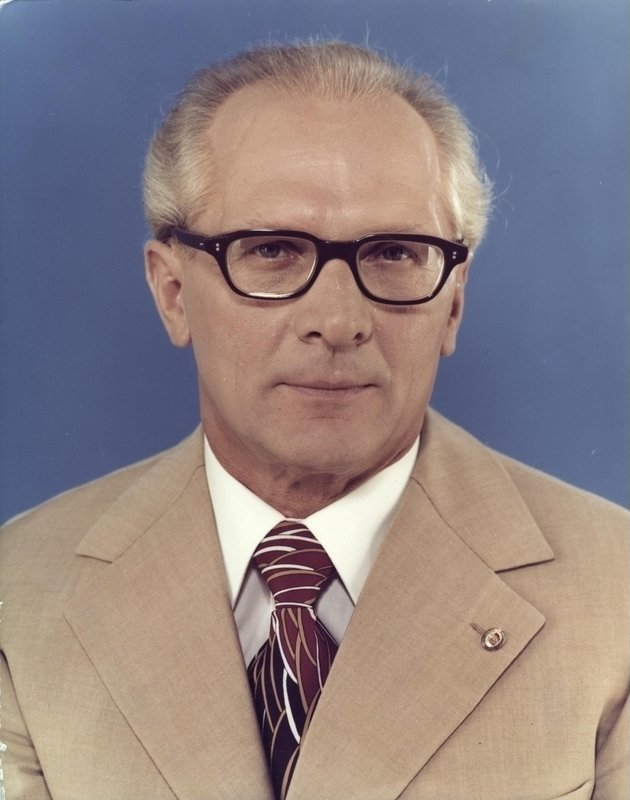
\includegraphics[width=0.3\textwidth]{Bilder/Erich_Honecker.jpg}
    \caption{Erich Honecker}
    Quelle: Wikipedia
    \label{img:honecker}
\end{figure}

Der Verlust Ulbrichts war ein tiefer Einschnitt für die DDR. Seine Veränderungen wurden nach seinem Abgang stark vernachlässigt und aus Schulbüchern und Chroniken entfernt. Sein Ziel der sozialistischen Wiedervereinigung Deutschlands wurde endgültig aufgegeben, indem entsprechende Hinweise aus der Verfassung gestrichen.

Weiterhin wurden viele Organisationen umbenannt und tragen statt \enquote{Deutschland} nun \enquote{DDR} im Namen. Um die emotionale Bindung zu einem Gesamtdeutschland aufrecht zu erhalten, prägte Honecker die Formulierung \enquote{Staatsangehörigkeit: DDR, Nationalität: deutsch}.\footcite{wiki:geschddr}


\subsection{Einheit von Wirtschafts- und Sozialpolitik}
\label{sub:wohnung}

Honeckers Amtszeit wurde gekennzeichnet durch den Beschluss der SED, die Hauptaufgabe der Politik müsse es sein, die Einheit von Wirtschafts- und Sozialpolitik zu erreichen. Dafür sollten der Lebensstandard und die Kaufkraft erhöht werden, wodurch eine bessere Zufriedenheit des Volkes und die Erhöhung der Arbeitskraft erreicht werden sollte.
Kernstück dieser Aufgabe war ein Wohnungsbauprogramm, welches das dringende Wohnungsproblem bis spätestens 1990 lösen sollte.
Im Rahmen dieses Projekts entstanden große Neubaugebiete mit - nach offiziellen Angaben - 3 Millionen komfortablen Wohnungen. Diese Zahlen waren allerdings geschönt, tatsächlich sind nur etwa 1,92 Millionen Wohnungen gebaut worden.
Da die Sanierung oder Abriss der alten Wohnungen zu teuer war, wurden diese einfach leer stehen gelassen. Dies führte zu einer starken Verödung der Städte.

Ein weiterer Schwerpunkt Honeckers Politik war die Beschaffung von westlichen Produktionsanlagen. Dafür wurden Kredite bei Banken der Bundesrepublik aufgenommen. Die DDR hatte damit erstmals hohe Auslandsschulden im nicht-sozialistischen Ausland. Einige sprachen schon damals vom möglichen \enquote{Anfang von Ende} der DDR.




\newpage



\section{Leben in der DDR}
\label{sec:leben}

\begin{quotation}
    \enquote{Wir mussten nur aus dem Fenster schauen, um zu sehen, wie alles, was in einem Lehrbuch [zum Sozialismus] steht, von der Realität widerlegt wird.} \\
    \it aus SPIEGEL Geschichte 3/2015: Die DDR - Leben im sozialistischen Deutschland
\end{quotation}

Als Erich Honecker im Mai 1971 an die Macht kam, versprach er seinem Volk ein besseres Land als es die DDR und das Gesamtdeutschland jemals waren. Dem Volk sollte es an nichts mangeln und die Kosten sollten gleich bleiben (dass dies unweigerlich zu einem Staatsbankrott führen musste, interessierte damals niemanden). 

Tatsächlich stiegen zu Beginn von Honeckers Amtszeit die Löhne und Rentenbeiträge, die Urlaubszeiten wurden verlängert, die Arbeitszeit verkürzt. Berufstätige Mütter konnten ein Jahr bei vollem Gehalt in eine \enquote{Babypause} gehen, die Kinderkrippen wurden ausgebaut, ...
Die Lebensqualität in der DDR erhöhte sich spürbar.

\subsection{Begrenzte Produktpalette}
\label{sub:begrenzt}

Aber die Preispoltik der DDR hatte auch ihre Schattenseiten. Durch die künstlich niedrig gehaltenen Mieten wurden größere und mehr Wohnungen gekauft, als man benötigte. Singles blieben auch nach der Scheidung in viel zu großen Wohnungen oder zogen um, aber behielten die Wohnung für schlechte Zeiten.
Selbiges spielte sich auch bei Lebensmitteln ab: Die Regierung schrieb für ein Brötchen einen Preis von 5 Pfenning fest. Dieser Preis lag weit unter den Produktionskosten der Bäcker. Da die Bäcker sich dadurch nicht mehr finanzieren konnten, wurde zu wenig produziert, um alle zu versorgen. Es kam durch die Preispolitik zu dem, was Honecker gerade vermeiden wollte: Zu einem permanenten Mangel. 

Alles, was gerade vorrätig war, wurde gekauft, egal ob man es brauchte oder nicht.
Manche Waren gab es nur zu bestimmten Zeiten, und dann waren sie innerhalb weniger Stunden ausverkauft.\footcite{spiegel:kap3}

Trotzdem wurden im Hintergrund die Produkte stark rationiert und viele Produkte gab es in der DDR einfach nicht.


\subsection{Unter Überwachung der Stasi - Ständige Angst}
\label{sub:stasi}

\enquote{
    Die meisten wissen nicht, was sie am 6. September oder am 28. Oktober 1984 gemacht haben. Hartmut Prößdorf schon. Er kann zum Teil minutiös auf seine Vergangenheit zurückblicken, ohne selbst Tagebuch geführt zu haben ‒ dank seiner Stasiakte. Am 24. April 1984 stellte der Luckenwalder einen Ausreiseantrag, genauer gesagt ein Übersiedlungsersuchen (ÜSE). "Wir waren damals zu dritt. Norbert Wegner, Edgar Gollnik und ich", berichtet Hartmut Prößdorf. Dass ein Ausreiseantrag gestellt wurde, war zu DDR-Zeiten nicht ungewöhnlich, dass aber gleich drei Leute zum Rat des Kreises kamen, weil sie die Republik verlassen wollten, das war ein Novum. "Den Tag werde ich nie vergessen", sagt der 61-Jährige. Seitdem wurde Hartmut Prößdorf bespitzelt und verhört.
} \\
\textit{aus maz-online.de: Rundum-Bewachung der Stasi} \\

\begin{figure}[hh]
    \centering
    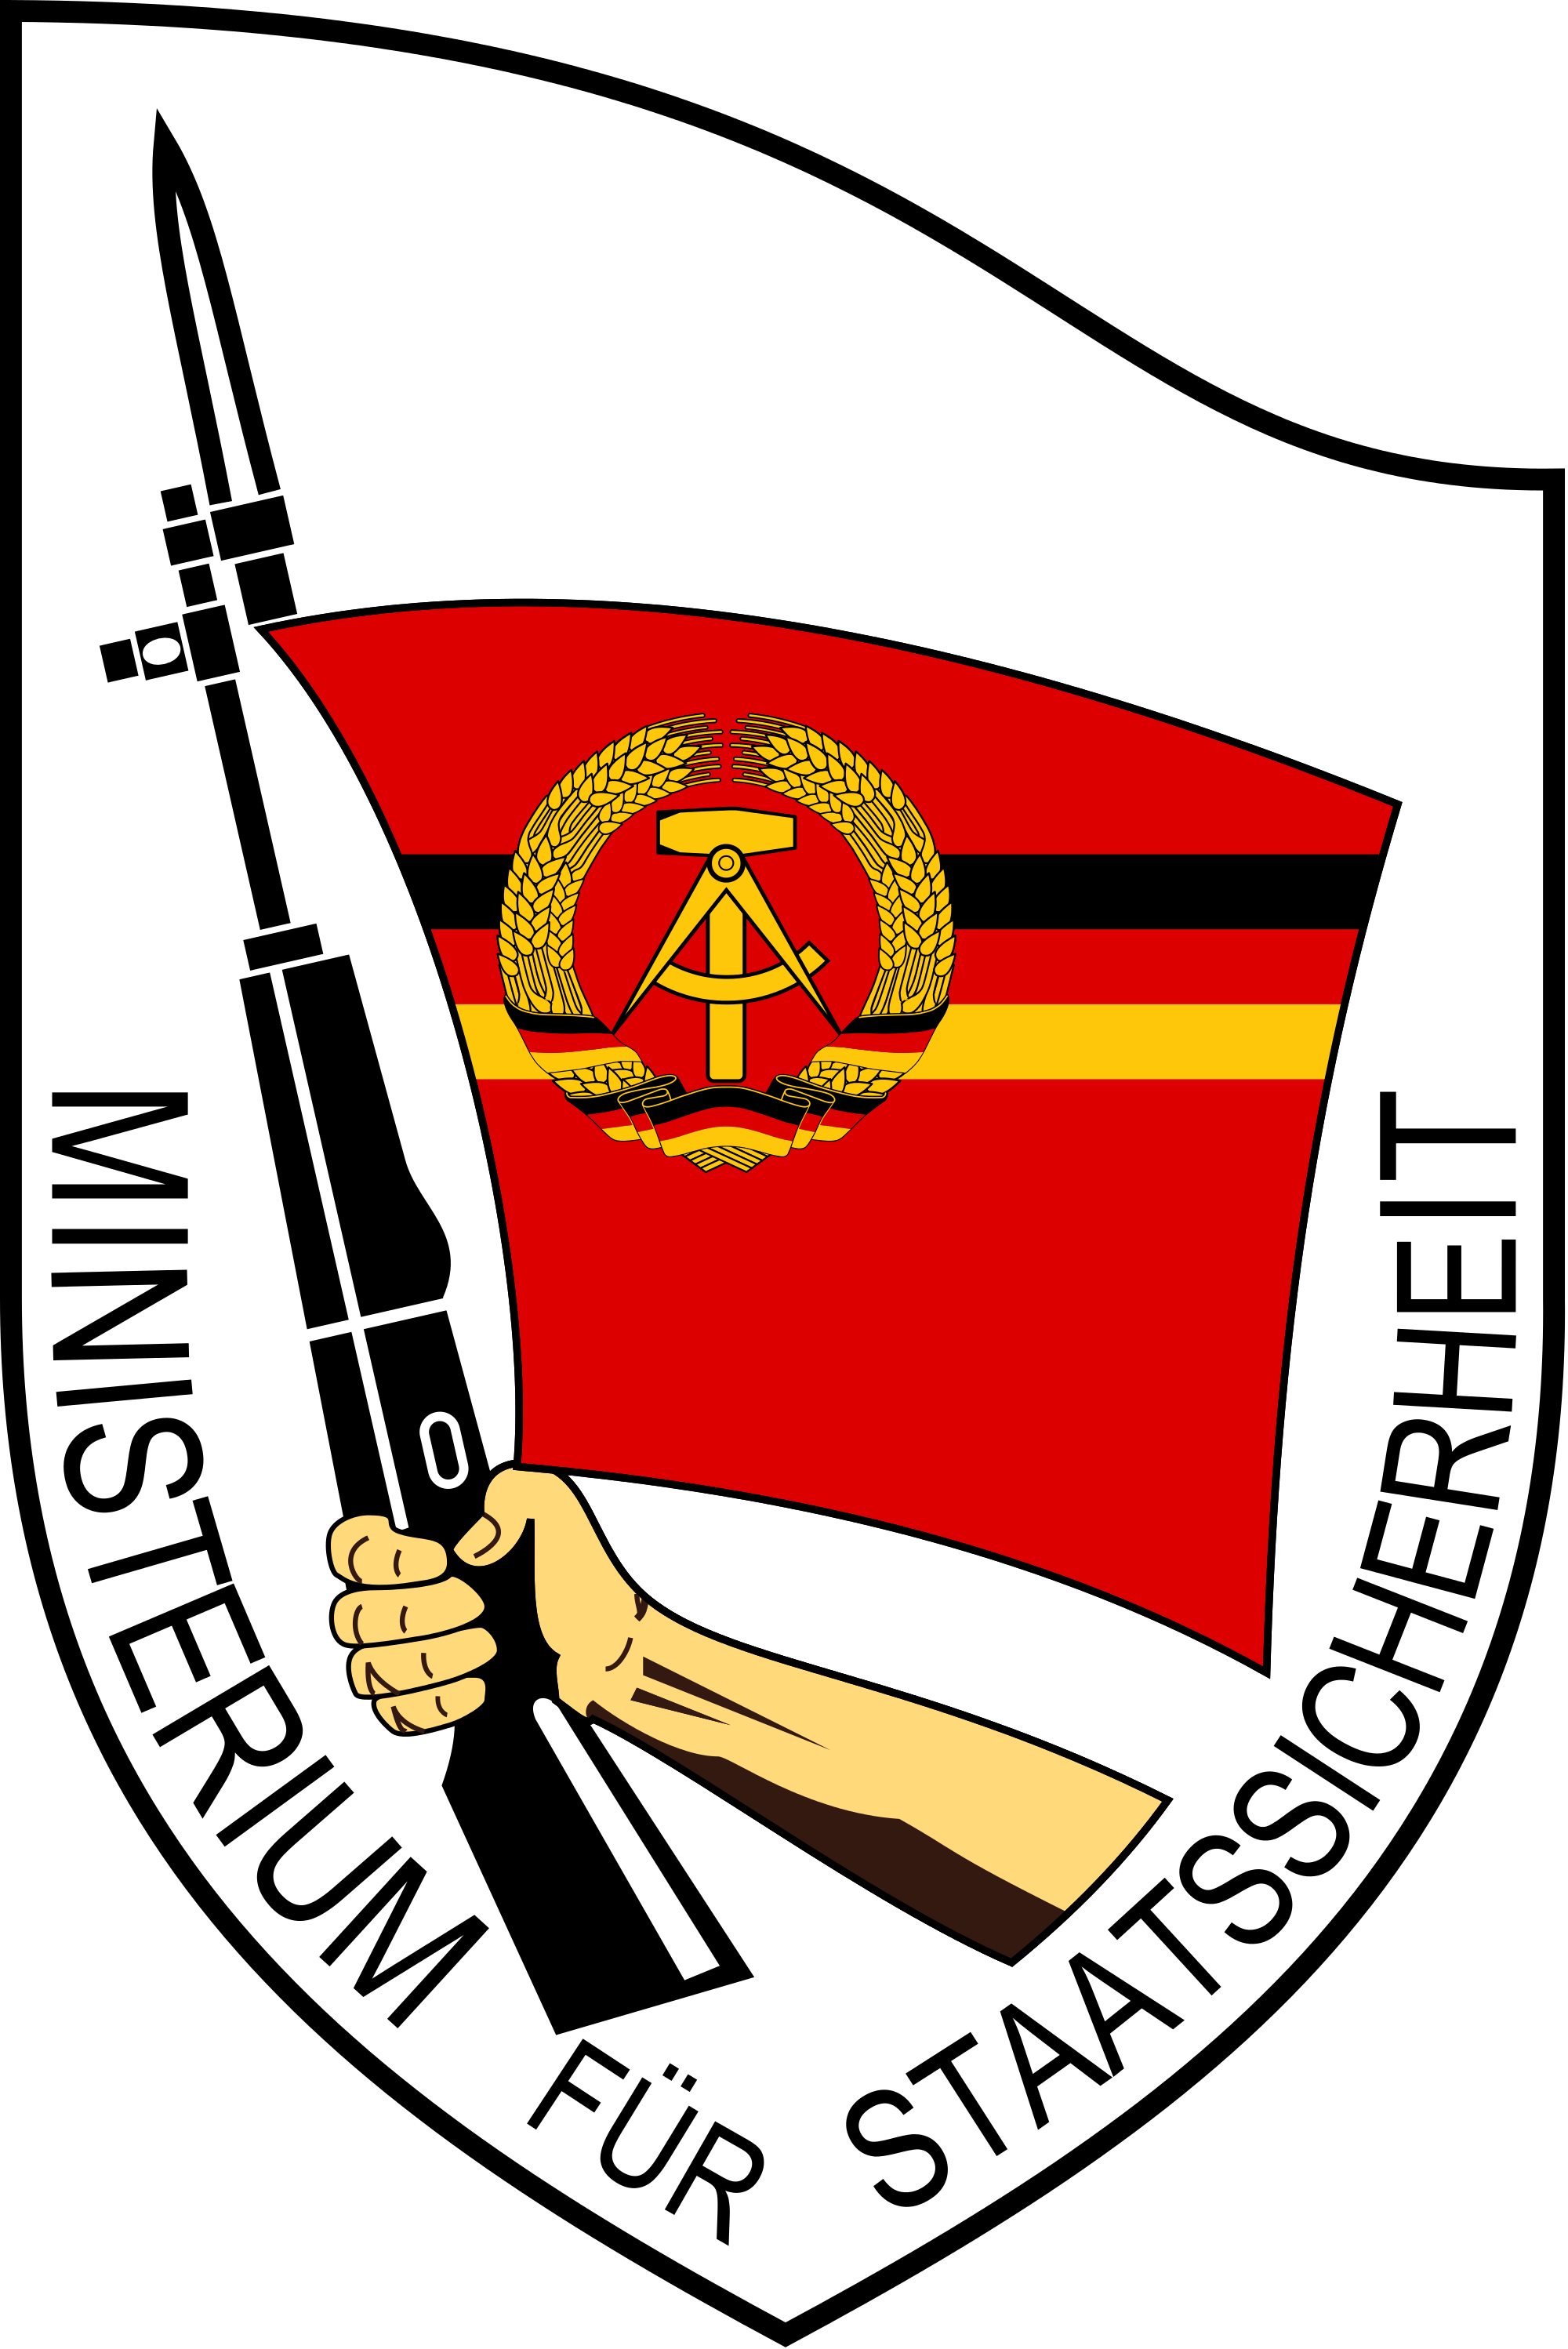
\includegraphics[width=0.5\textwidth]{Bilder/Emblem_Stasi.png}
    \caption{Emblem des Ministeriums für Staatssicherheit}
    Quelle: Wikipedia
    \label{img:stasi}
\end{figure}

In der DDR konnte man sich nie sicher sein, \textbf{alleine} zu sein. Man musste ständig damit rechnen, dass man durch das Ministerium für Staatsicherheit (kurz: Stasi) bespitzelt zu werden. Das MfS war das Schutzschild der SED eine geheime Parteipolizei, die jegliche Form der Opposition aufspüren und unterdrücken sollte.
Da das MfS nicht der Regierung, sondern nur der SED unterstand, agierte das MfS fernab jeglicher Rechtsstaatlichkeit.

Das MfS beschäftigte 1989 genau 91.015 hauptamtliche Mitarbeiter. Der Hauptbestandteil des MfS bestand aber aus Inoffiziellen Mitarbeitern, also im Prinzip jedermann. Man wusste nicht, ob der eigene Vater oder der Geschäftskollege bei der Stasi war, weshalb die Menschen sich nicht mehr trauten, etwas gegen die aktuelle Poitik der SED zu sagen.
Zum Ende der DDR waren etwa 189.000 Inoffizielle Mitarbeiter gelistet.\footcite{izpb:schein}


\newpage



\section{Das Ende der DDR (1981 - 1990)}
\label{sec:das-ende-der-ddr}

\subsection{Finanzkrise}
\label{finanzkrise}

Die UdSSR kam durch die hohen Kosten des Klaten Krieges in eine kritische wirtschaftliche Lage, weshalb sie die Preise für Exporte drastisch erhöhte. Dies bekam auch die DDR zu spüren, da sie eine hohe Abhängigkeit zur Sowjetunion hatte.
Da auch Öllieferungen gekürzt wurden (von 19 auf 17 Millionen Tonnen), brach die größte Devisenquelle der DDR zusammen, Die DDR konnte erstmals Kredite und Zinsen nur durch die Aufnahme neuer Kredite zurückzahlen. Vor allem mit den westlichen Kreditinstituten kam es schnell zu Problemen.

Die Bundesrepublik übernahm Kredite im Wert von einer Milliarde D-Mark von der DDR, um deren Stabilität zu wahren.
Die DDR musste im Gegenzug die Selbstschussanlagen an der innerdeutschen Grenze abbauen und Westdeutschen die Einreise erleichtern. \\

Bereits Ende der 1980er-Jahre wurde der wirstchaftliche Verfall der DDR sichtbar, als sie Neuinvestitionen und Reperaturen nicht mehr zahlen konnten. Unter anderem der Wohnungsbau (siehe S. \pageref{sub:wohnung}) führte 1989 in eine kritische Situation. 
Reformvorschläge Honeckers wurden konsequent abgelehnt.

Dies führte zu einem Zwang mit der Bundesrepublik zu verhandeln, die Gunst dieser Verhandlungen lag immer mehr auf der Seite der BRD.


\subsection{Ausreisewelle}
\label{ausreise}

1984 gab es außerordentlich viele Umsiedlungen in die Bundesrepublik (etwa 40.000 Menschen\footcite{wiki:geschddr}). Ausreisewillige flüchteten in die Deutsche Botschaft nach Prag oder in die Botschaft der BRD in Westberlin, wodurch sie eine prioritisierte Abarbeitung ihrer Anträge erreichen konnten.

Als im Mai 1989 Ungarn seine Grenzen zu Österreich abbaute, versuchten hunderte DDR-Bürger über Ungarn in den Westen zu gelangen, Botschaften und DDR-Grenzen mussten daraufhin wegen Überfüllung geschlossen werden.
Flüchtige, die sich zu diesem Zeitpunkt bereits außerhalb des DDR-Gebiets aufhielten, durften in die Bundesrepublik ausreisen.


\subsection{Montagsdemonstrationen in Leipzip}[hh]

\begin{figure}[hbp]
    \centering
    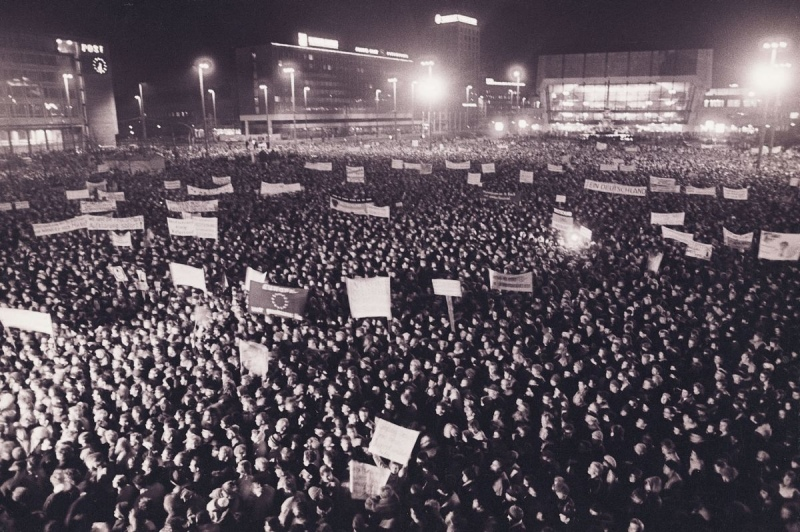
\includegraphics[width=\textwidth]{Bilder/montagsdemo.jpg}
    \caption{Montagsdemonstration vom 9. Oktober 1989}
    Quelle: \url{http://leipzig.travel}
    \label{img:demo}
\end{figure}

Seit dem 4. September 1989 wurden in Leipzig wöchentliche friedliche Montagsdemonstrationen abgehalten. Die größte Demonstration der DDR mit über einer Million Teilnehmern fand am 4. November 1989 statt, diese wurde sogar live im Fernsehen übertragen. Auch der bekannte Spruch

\begin{quotation}
    \enquote{\bf Wir sind das Volk}
\end{quotation}

wurde am 7. Oktober mit 70.000 Teilnehmern das erste Mal ausgerufen. Honecker wurde daraufhin zum Rücktritt von allen Ämtern gezwungen. 

Landesweit wurden Proteste am 40. Jahrestag der DDR abgehalten.


\subsection{Gründung von Oppositionsbewegungen}

Im Herbst 1989 kam es zur Gründung vieler neuer Oppositionsbewegungen, die Zweifel an der Führungsrolle der SED äußerten.

Am 7. November 1989 trat die gesamte Regierung und das Politbüro zurück.


\subsection{Die Rede Günter Schabowskis}

\begin{figure}[hh]
    \centering
    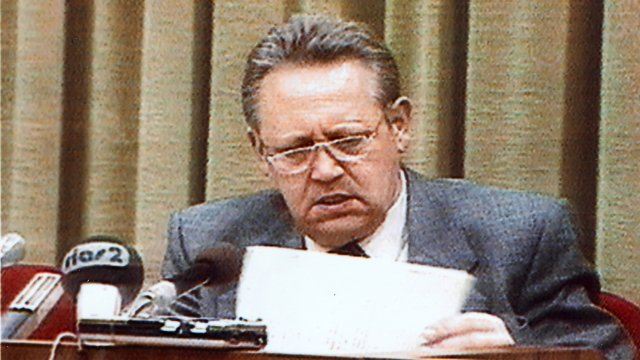
\includegraphics[width=0.7\textwidth]{Bilder/Schabowski.jpg}
    \caption{Günter Schabowski am 9. Nov. 1989}
    Quelle: SPIEGEL Online
    \label{img:schabowski}
\end{figure}

Günter Schabowski referierte am 9. November 1989 über die zehnte Tagung des Zentralkomitees der SED. Nach fast einer Stunde war sein Monolog zu Ende und es wurden Fragen durch die Journalisten gestellt. Der italiensiche Reporter Ricciardo Ehrmann stellte die verhängnisvolle Frage über das neu beschlossene Reisegesetz. Schabowskis Antwort belief sich auf einige Minuten, an deren Ende fieel der Satz: \textit{\enquote{Deshalb haben wir uns dazu entschlossen, heute eine Regelung zu treffen, die es jedem Bürger der DDR möglich macht, über Grenzübergangspunkte der DDR auszureisen.}}

Ein Reporter der \enquote{BILD}-Zeitung, hakte nach, ab wann das neue Gesetz gelten solle. Schabowski blätterte in der ihm direkt von der Pressekonferenz überreichte Mappe und übersah dabei die \textbf{Sperrfrist} dieser Information bis zum nächsten Morgen. Er stotterte:

\begin{quotation}
    \enquote{Nach meiner Kenntnis  ist das sofort, unverzüglich}
\end{quotation}


\subsection{Der Fall der Mauer}

\begin{figure}[hh]
    \centering
    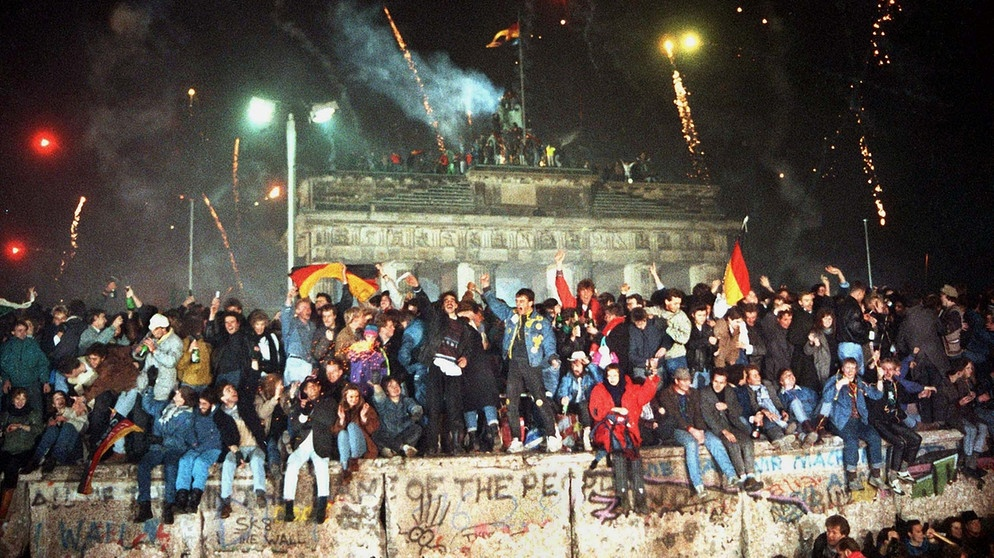
\includegraphics[width=0.5\textwidth]{Bilder/mauerfall.jpg}
    \caption{Menschen feiern den Fall der Mauer}
    Quelle: Bayrischer Rundfunk
    \label{img:mauerfall}
\end{figure}

Durch diesen Kommunikationsfehler war bereits nach wenigen Minuten in allen Fernseh- und Radiosendern die Meldung der \enquote{Öffnung} der Grenzen zu sehen und zu hören. Die Menschen strömten zu den Grenzen und versuchten, in die Bundesrepublik zu gelangen. Da die Grenzsoldaten nichts von der (noch nicht) geplanten Öffnung der Grenzen wussten, forderten die Menschen die Öffnung unter Berufung auf das SED-Politbüro.

Die Grenzsoldaten konnten dem Sturm nicht lange standhalten und öffneten die Grenzen tatsächlich. Die Mauer war gefallen.\footcite{spiegel:schabowski}\footcite{youtube:schabowski}


\subsection{Wiedervereinigung}

Im Dezember 1989 wurde die Führungsrolle der SED aus der Verfassung gestrichen und Verfahren gegen ehemalige Partei-Funktionäre ermittelt.
Der SED-Genralsekretär und Staatsratsvorsitzende Egon Krenz trat von allen Ämtern zurück.

Es wurde erstmals ein Runder Tisch mit den Oppositionsgruppen gebildet, erstmals wurde due Politik durch nichtgewählte Vertreter des Volkes mitbestimmt.

Nach dem Mauerfall änderte sich das Motto der noch immer stattfindenden Montagsdemonstrationen. Es wurde nun mit dem Leitspruch \textit{\enquote{Wir sind \bf EIN Volk}} die Wiedervereinigung Deutschlands gefordert.

Im Februar 1990 sprachen Helmut Kohl und Michail Gorbatschow öffentlich über eine mögliche Wiederverinigung Deutschlands. Am 18. März wurde die erste Freie Volkskammer in Wahlen, die geltenden Richtlinien entsprechen, gewählt.

Am 1. Juli 1990 trat die \textit{Währungs-, Wirtschafts- und Sozialunion} mit der Bundesrepublik inkraft.

Am 31. August wurde der Einigungsvertrag durch die Bundesrepublik und die DDR unterzeichnet. Die Aliierten stimmten diesem am 12. September zu.

Seit dem 3. Oktober 1990 ist Deutschland wiedervereint. Die Existenz der DDR erlosch mit diesem Zeitpunkt als Staat und Völkerrechtssubjekt.

\begin{figure}[h]
    \centering
    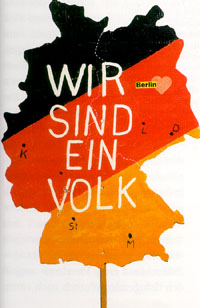
\includegraphics[width=0.3\textwidth]{Bilder/einvolk.jpg}
    \caption{Wir sind ein Volk}
    Quelle: \url{http://www.lawrencreglatz.com}
    \label{img:einvolk}
\end{figure}





\newpage



\listoffigures



\newpage



\printbibliography
\end{document}
